\documentclass[11pt]{article}
\usepackage[margin=1in]{geometry}
\usepackage{graphicx}
\usepackage{booktabs}
\usepackage{float}
\usepackage{hyperref}
\title{CS728 PA2 Report: Training Dynamics of RNNs and GRUs}
\author{22b1205,22b0955,22b1205}
\date{\today}
\begin{document}
\maketitle

\section{Experimental Setup}
All required runs were executed with the exact assignment commands and shared hyperparameters:
\begin{verbatim}
--nhid 50 --lr 0.01 --bs 20 --min_length 50 --max_length 200
--maxiters 50000 --ebs 10000 --cbs 1000 --checkFreq 20
--seed 52 --valid_seed 12345 --collectDiags --diagBins 60 --satThresh 0.05
\end{verbatim}

\section{Run Summary}
\begin{table}[H]
\centering
\begin{tabular}{lrrrrrr}
\toprule
Run & Best valid err(\%) & Last valid err(\%) & Last $\rho$ & Mean log10($g_t$) & Mean sat & z/r sat \\
\midrule
A1 & 100.0000 & 100.0000 & 14.1958 & -4.1731 & 0.0168 & N/A \\
A2 & 100.0000 & 100.0000 & 1.1389 & -4.5623 & 0.6280 & N/A \\
A3 & 100.0000 & 100.0000 & 1.1194 & -4.5137 & 0.6105 & N/A \\
A4 & 100.0000 & 100.0000 & 2.0123 & -6.2960 & 0.5382 & 0.1818/0.4556 \\
A5 & 100.0000 & 100.0000 & 1.2943 & -4.3039 & 0.8498 & 0.1246/0.4925 \\
B1 & 25.9000 & 39.6000 & 0.7051 & -11.9535 & 0.9386 & N/A \\
B2 & 24.2500 & 39.1800 & 0.0808 & -11.9574 & 0.9947 & 0.1193/0.4989 \\
\bottomrule
\end{tabular}
\caption{Numerical summary from final checkpoints.}
\end{table}

\section{Per-run Plots and Observations}
For each run, we include only: (i) histogram of $\log_{10}\|\partial L/\partial h_t\|$, (ii) hidden saturation-distance histogram, and (iii) validation curve.

\subsection{A1}

\begin{figure}[H]
\centering
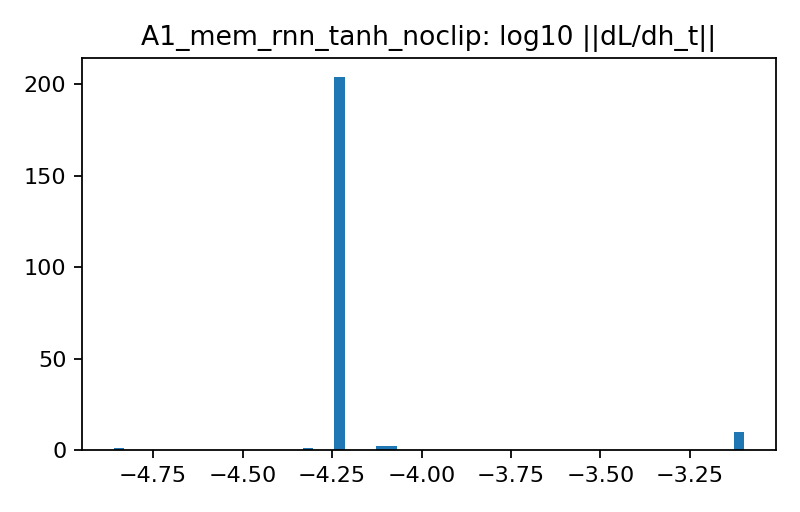
\includegraphics[width=0.48\textwidth]{../runs/figures/A1_mem_rnn_tanh_noclip_grad_hist.png}
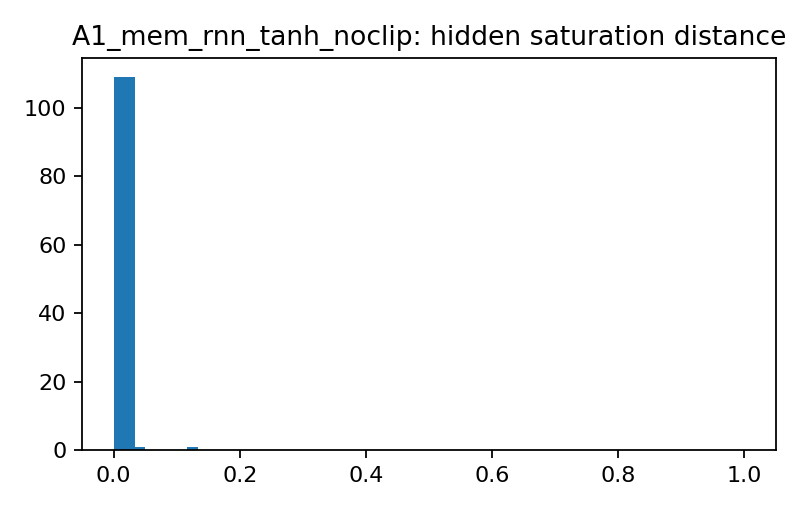
\includegraphics[width=0.48\textwidth]{../runs/figures/A1_mem_rnn_tanh_noclip_sat_hist.png}
\caption{Gradient-through-time and hidden saturation histograms.}
\end{figure}

\begin{figure}[H]
\centering
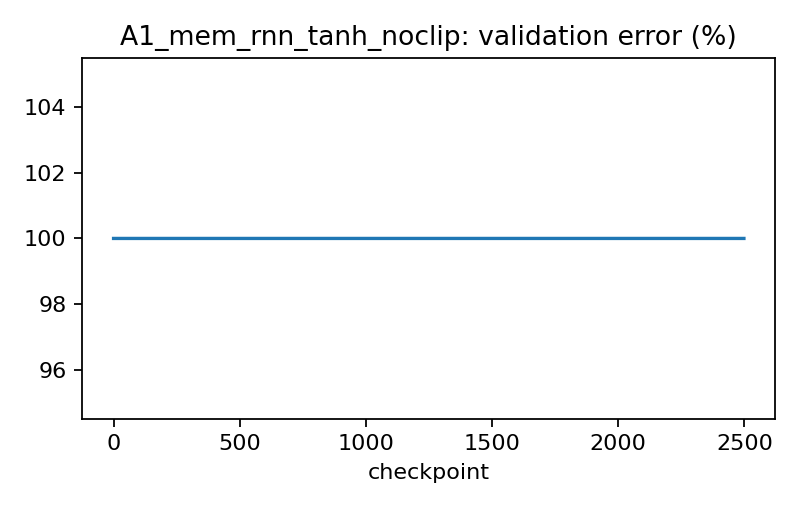
\includegraphics[width=0.62\textwidth]{../runs/figures/A1_mem_rnn_tanh_noclip_valid_curve.png}
\caption{Validation error (\%) over checkpoints.}
\end{figure}
\paragraph{Observation}
The gradient histogram is less left-shifted than most other memorization runs, so gradients are less vanishing at many timesteps. The hidden saturation-distance histogram is concentrated near 0, indicating heavy tanh saturation. The validation-error curve remains near 100\%, so sequence-level memorization performance does not improve.

\subsection{A2}

\begin{figure}[H]
\centering
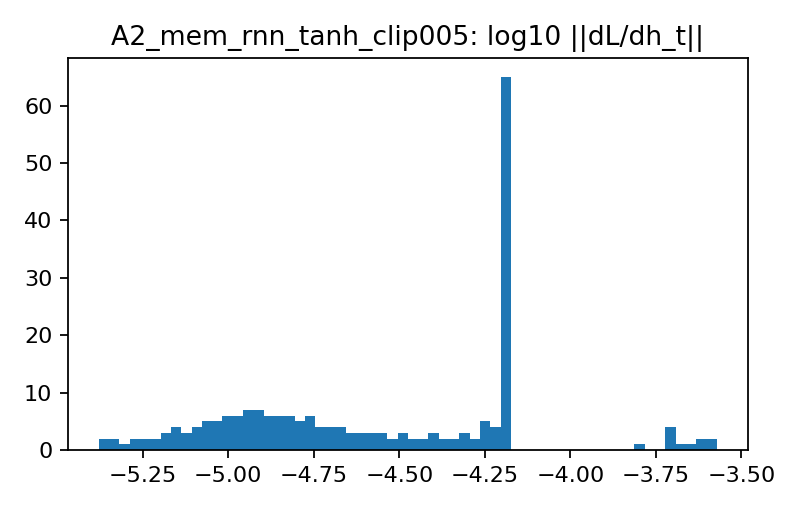
\includegraphics[width=0.48\textwidth]{../runs/figures/A2_mem_rnn_tanh_clip005_grad_hist.png}
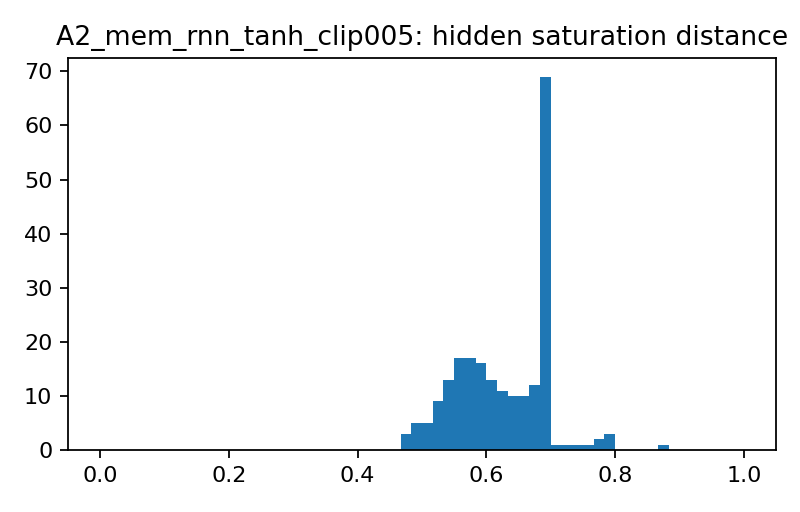
\includegraphics[width=0.48\textwidth]{../runs/figures/A2_mem_rnn_tanh_clip005_sat_hist.png}
\caption{Gradient-through-time and hidden saturation histograms.}
\end{figure}

\begin{figure}[H]
\centering
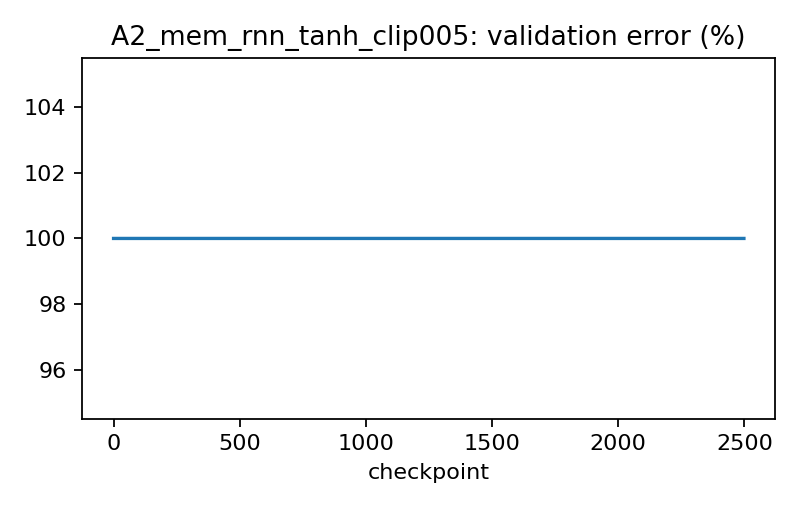
\includegraphics[width=0.62\textwidth]{../runs/figures/A2_mem_rnn_tanh_clip005_valid_curve.png}
\caption{Validation error (\%) over checkpoints.}
\end{figure}
\paragraph{Observation}
Compared to A1, the gradient histogram is shifted left (more negative values), and hidden saturation distance is much larger (less hidden saturation). The validation-error curve still stays near 100\%, so this does not translate to sequence-level success on memorization.

\subsection{A3}

\begin{figure}[H]
\centering
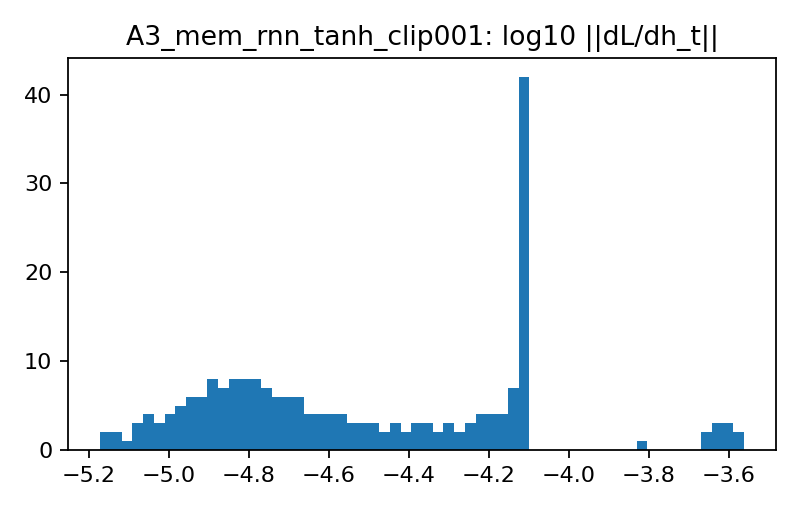
\includegraphics[width=0.48\textwidth]{../runs/figures/A3_mem_rnn_tanh_clip001_grad_hist.png}
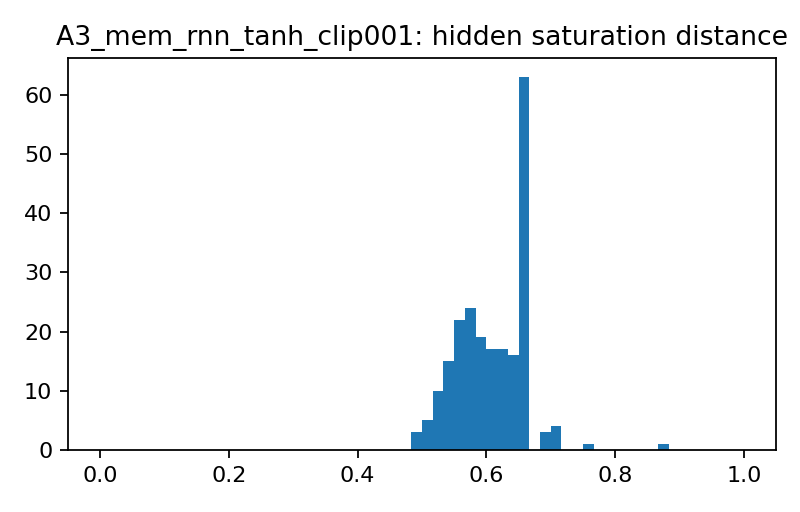
\includegraphics[width=0.48\textwidth]{../runs/figures/A3_mem_rnn_tanh_clip001_sat_hist.png}
\caption{Gradient-through-time and hidden saturation histograms.}
\end{figure}

\begin{figure}[H]
\centering
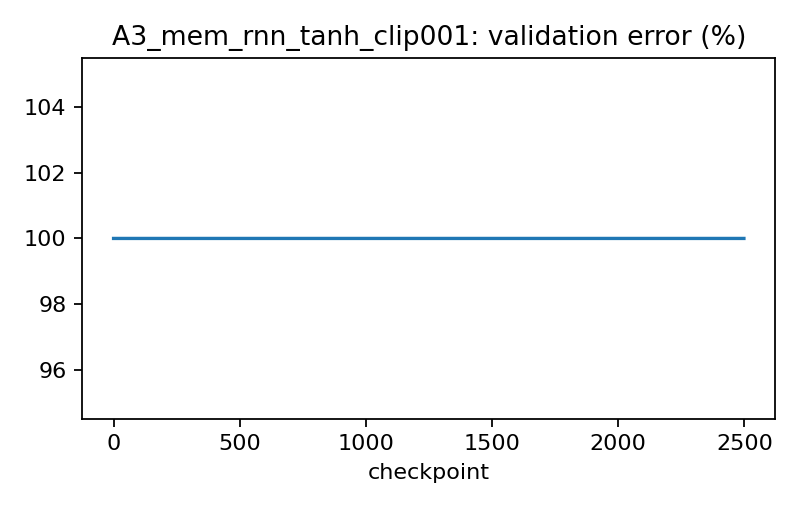
\includegraphics[width=0.62\textwidth]{../runs/figures/A3_mem_rnn_tanh_clip001_valid_curve.png}
\caption{Validation error (\%) over checkpoints.}
\end{figure}
\paragraph{Observation}
This run is similar to A2: gradient values are mostly in the vanishing side, while hidden saturation distance remains high (little hidden saturation). The validation-error curve remains near 100\%, so no practical memorization gain is visible.

\subsection{A4}

\begin{figure}[H]
\centering
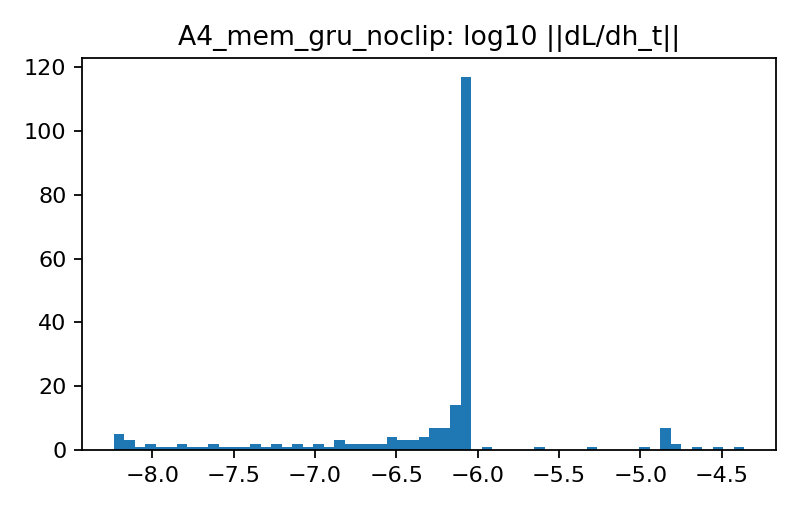
\includegraphics[width=0.48\textwidth]{../runs/figures/A4_mem_gru_noclip_grad_hist.png}
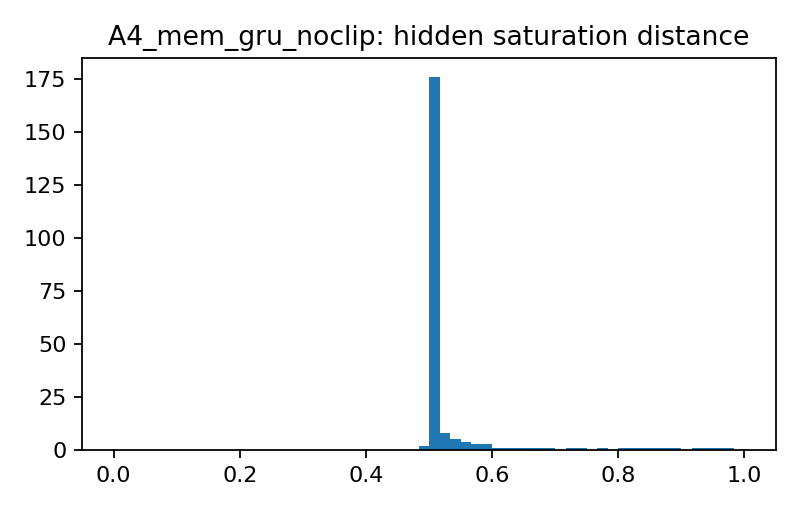
\includegraphics[width=0.48\textwidth]{../runs/figures/A4_mem_gru_noclip_sat_hist.png}
\caption{Gradient-through-time and hidden saturation histograms.}
\end{figure}

\begin{figure}[H]
\centering
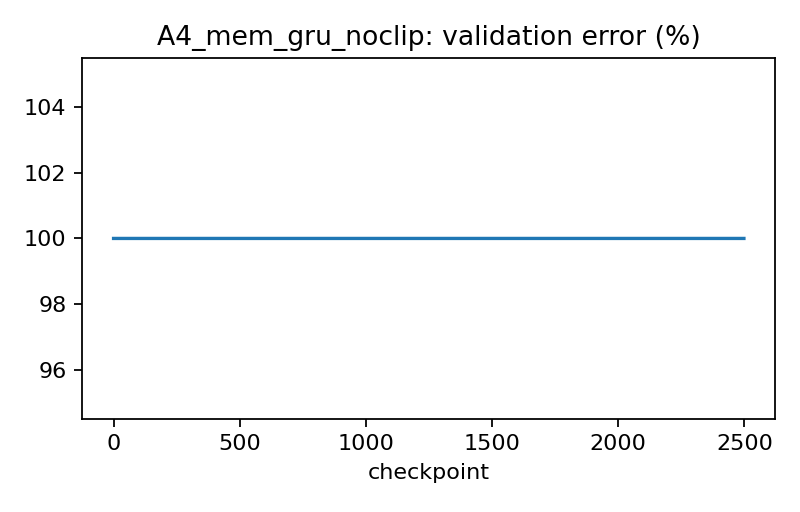
\includegraphics[width=0.62\textwidth]{../runs/figures/A4_mem_gru_noclip_valid_curve.png}
\caption{Validation error (\%) over checkpoints.}
\end{figure}

\begin{figure}[H]
\centering
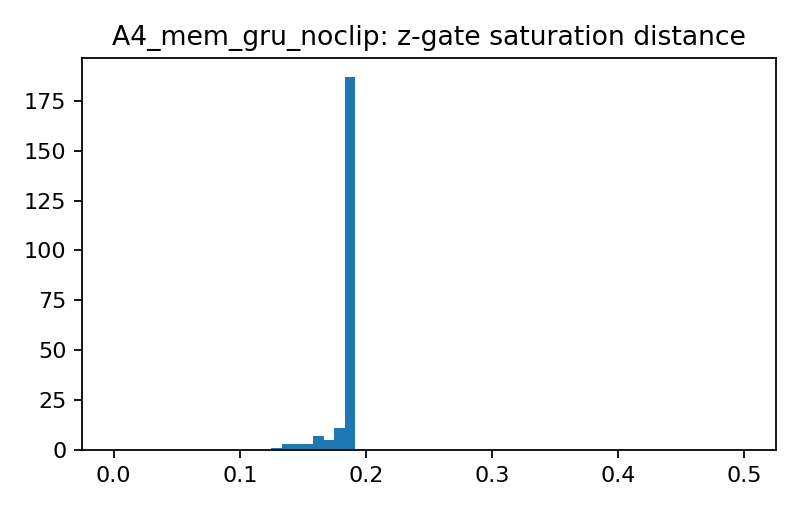
\includegraphics[width=0.48\textwidth]{../runs/figures/A4_mem_gru_noclip_zsat_hist.png}
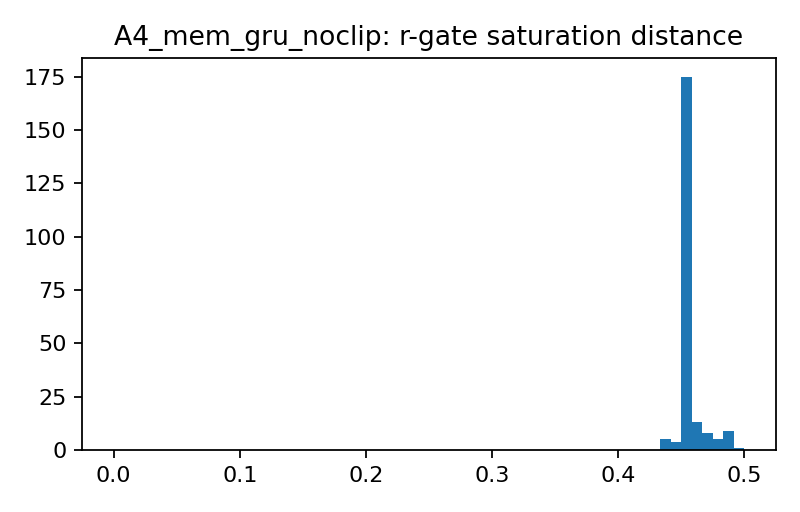
\includegraphics[width=0.48\textwidth]{../runs/figures/A4_mem_gru_noclip_rsat_hist.png}
\caption{GRU gate saturation-distance histograms (update and reset gates).}
\end{figure}
\paragraph{Observation}
For GRU without clipping, the gradient histogram is strongly left-shifted (vanishing-through-time behavior). Hidden saturation is moderate. In gate plots, update-gate distances are lower (more saturation) while reset-gate distances are closer to 0.5 (less saturation). The validation-error curve remains near 100\%.

\subsection{A5}

\begin{figure}[H]
\centering
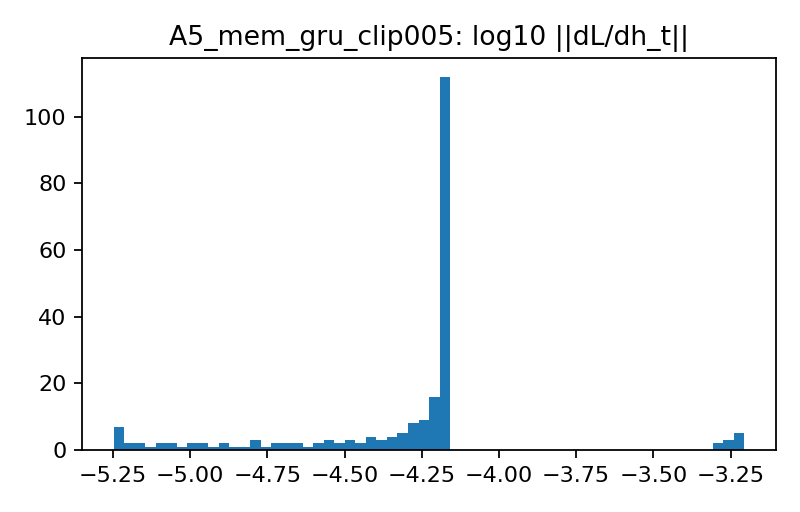
\includegraphics[width=0.48\textwidth]{../runs/figures/A5_mem_gru_clip005_grad_hist.png}
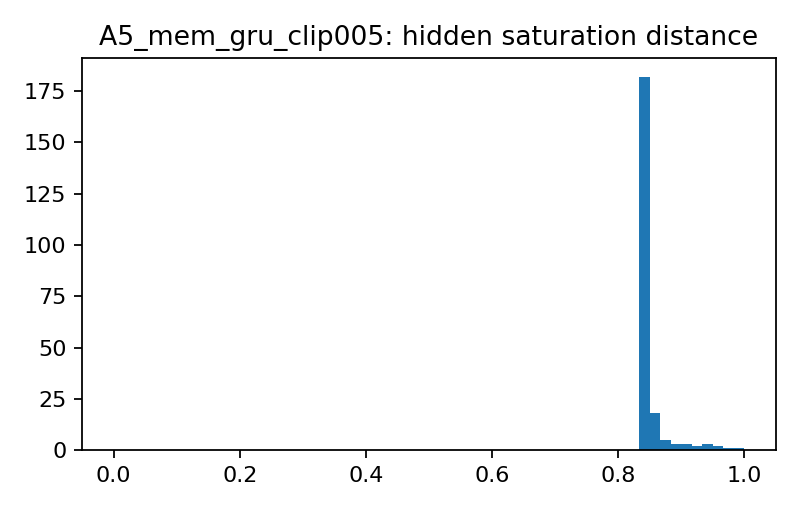
\includegraphics[width=0.48\textwidth]{../runs/figures/A5_mem_gru_clip005_sat_hist.png}
\caption{Gradient-through-time and hidden saturation histograms.}
\end{figure}

\begin{figure}[H]
\centering
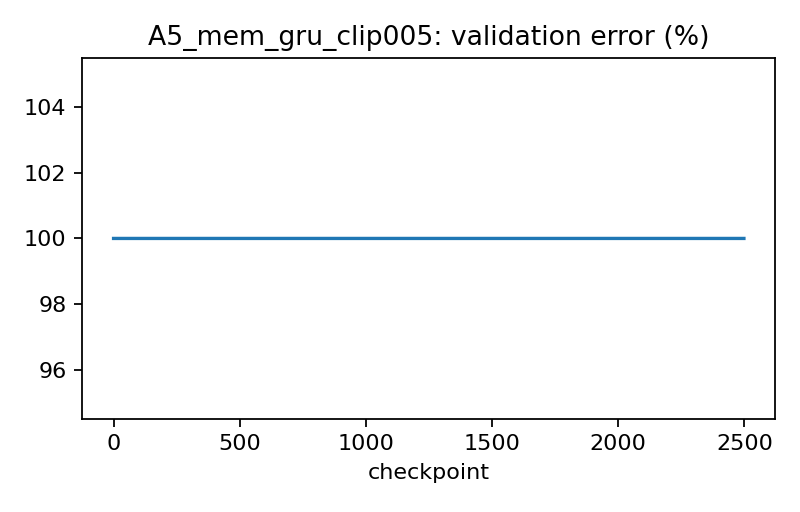
\includegraphics[width=0.62\textwidth]{../runs/figures/A5_mem_gru_clip005_valid_curve.png}
\caption{Validation error (\%) over checkpoints.}
\end{figure}

\begin{figure}[H]
\centering
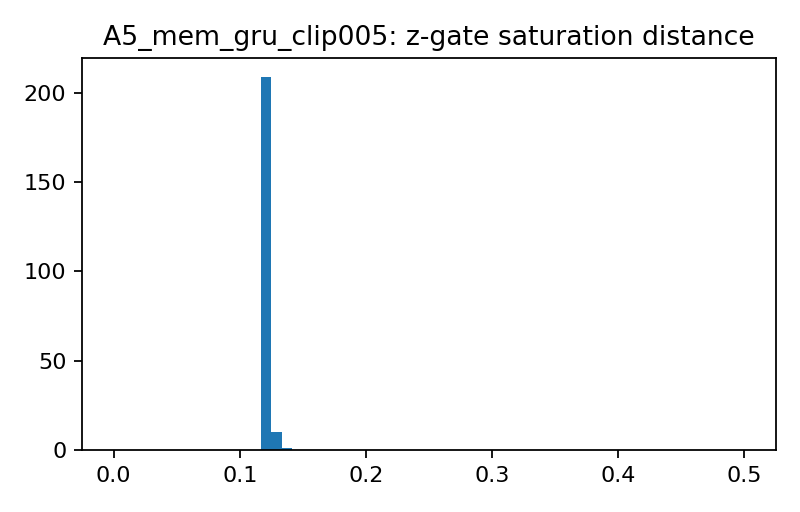
\includegraphics[width=0.48\textwidth]{../runs/figures/A5_mem_gru_clip005_zsat_hist.png}
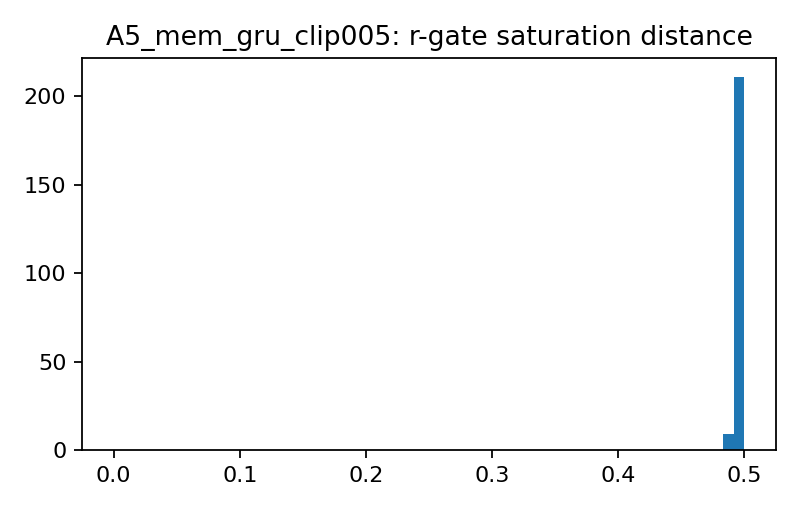
\includegraphics[width=0.48\textwidth]{../runs/figures/A5_mem_gru_clip005_rsat_hist.png}
\caption{GRU gate saturation-distance histograms (update and reset gates).}
\end{figure}
\paragraph{Observation}
With clipping enabled, the gradient histogram shifts right compared with A4 (less vanishing), and hidden saturation distance is very high (hidden states far from tanh saturation). Gate histograms still show update gate more saturated than reset gate. Despite these changes, the validation-error curve is still near 100\%.

\subsection{B1}

\begin{figure}[H]
\centering
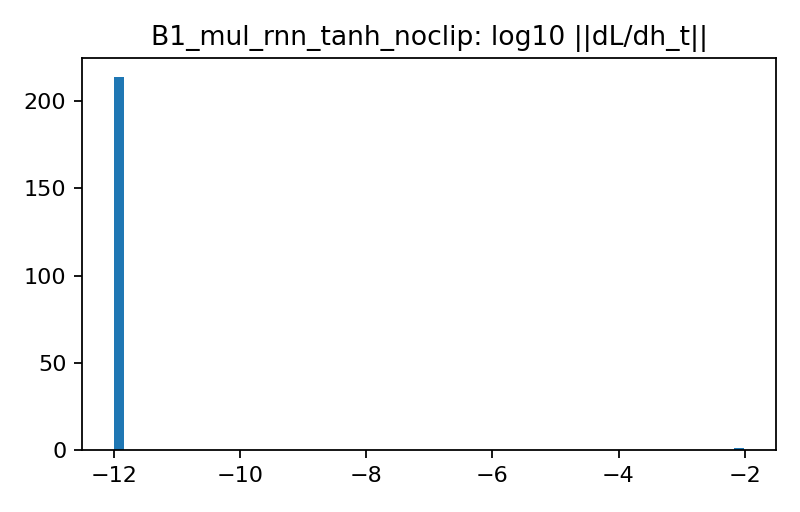
\includegraphics[width=0.48\textwidth]{../runs/figures/B1_mul_rnn_tanh_noclip_grad_hist.png}
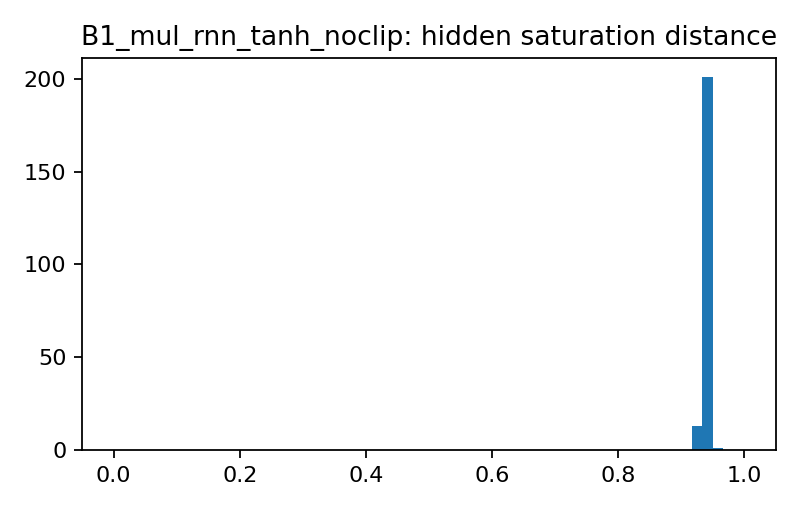
\includegraphics[width=0.48\textwidth]{../runs/figures/B1_mul_rnn_tanh_noclip_sat_hist.png}
\caption{Gradient-through-time and hidden saturation histograms.}
\end{figure}

\begin{figure}[H]
\centering
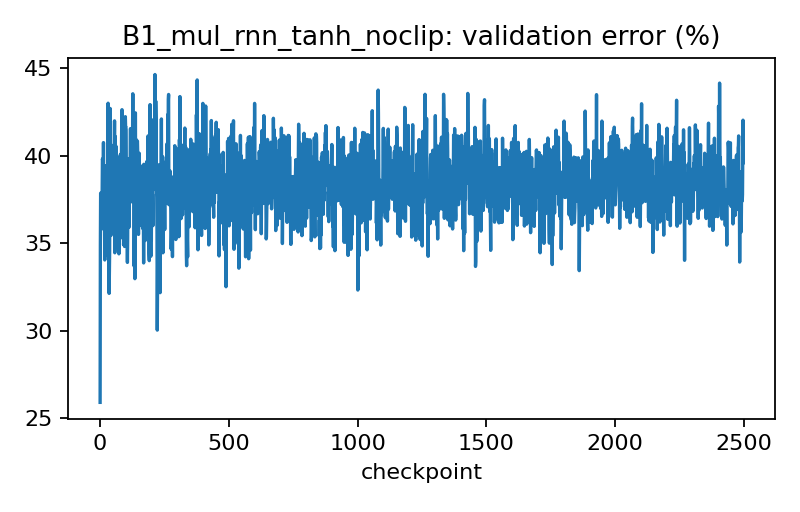
\includegraphics[width=0.62\textwidth]{../runs/figures/B1_mul_rnn_tanh_noclip_valid_curve.png}
\caption{Validation error (\%) over checkpoints.}
\end{figure}
\paragraph{Observation}
On multiplication with vanilla RNN, the gradient histogram is extremely left-shifted (strong vanishing). Hidden saturation distance is very high, so hidden units are generally not tanh-saturated. The validation-error curve has  25.9\% best error which is achieved initially then it just oscillates.

\subsection{B2}

\begin{figure}[H]
\centering
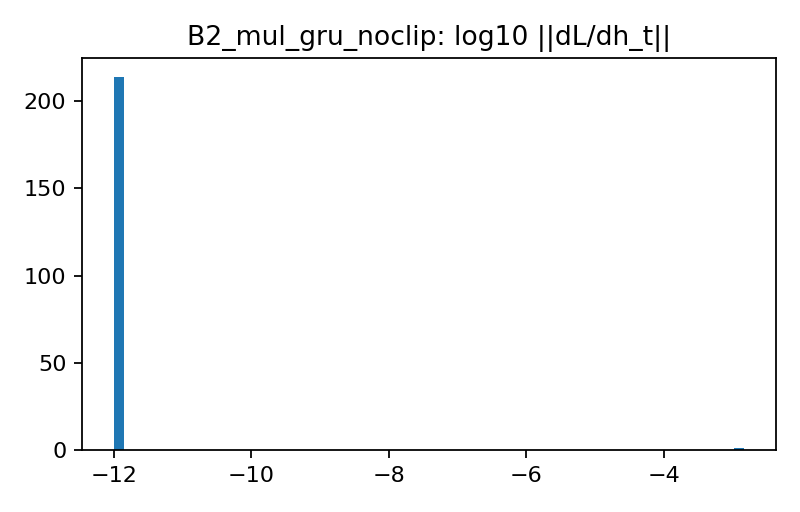
\includegraphics[width=0.48\textwidth]{../runs/figures/B2_mul_gru_noclip_grad_hist.png}
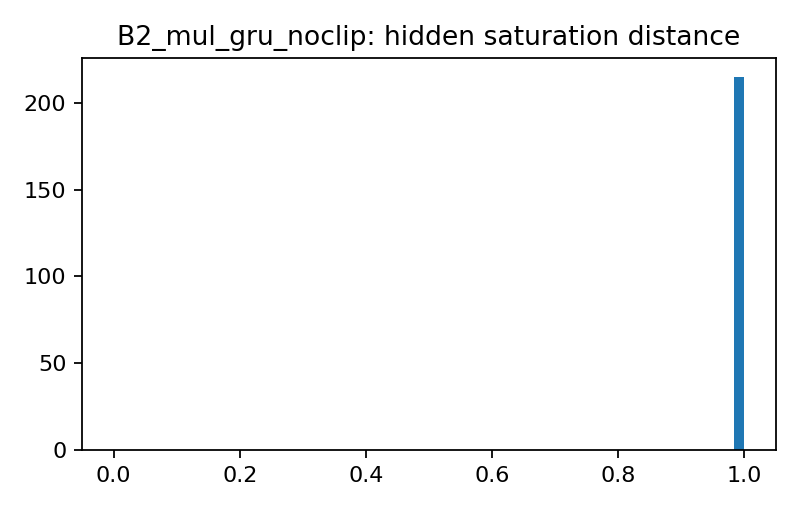
\includegraphics[width=0.48\textwidth]{../runs/figures/B2_mul_gru_noclip_sat_hist.png}
\caption{Gradient-through-time and hidden saturation histograms.}
\end{figure}

\begin{figure}[H]
\centering
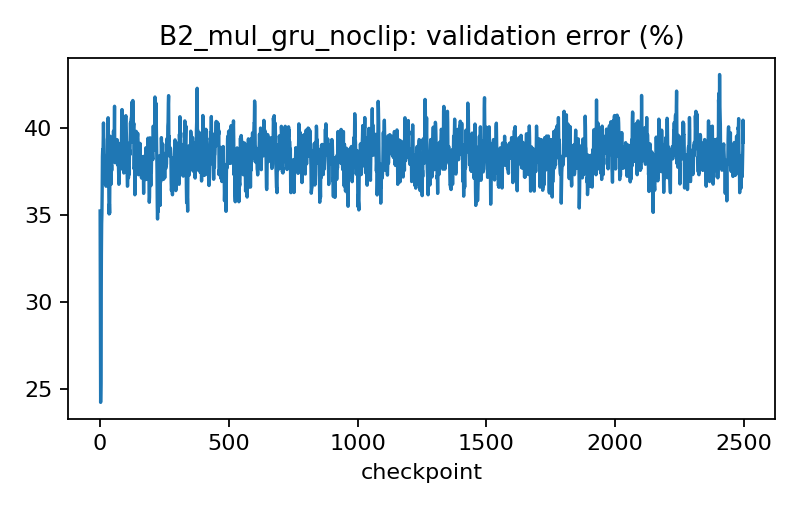
\includegraphics[width=0.62\textwidth]{../runs/figures/B2_mul_gru_noclip_valid_curve.png}
\caption{Validation error (\%) over checkpoints.}
\end{figure}

\begin{figure}[H]
\centering
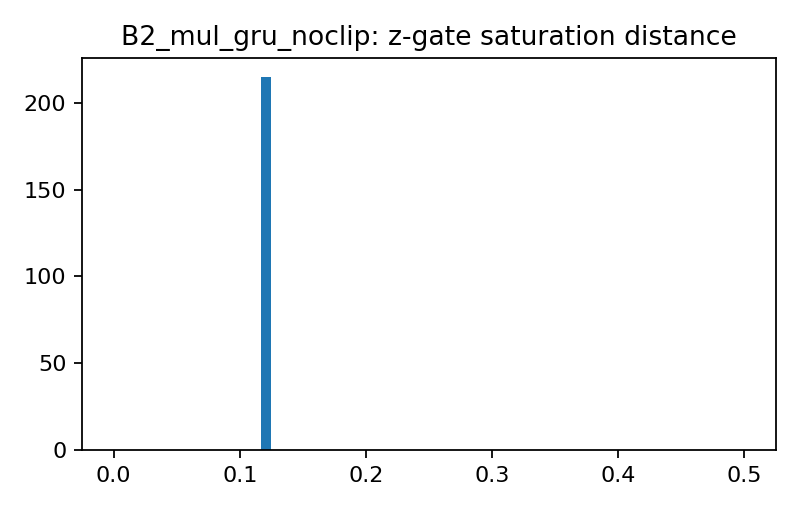
\includegraphics[width=0.48\textwidth]{../runs/figures/B2_mul_gru_noclip_zsat_hist.png}
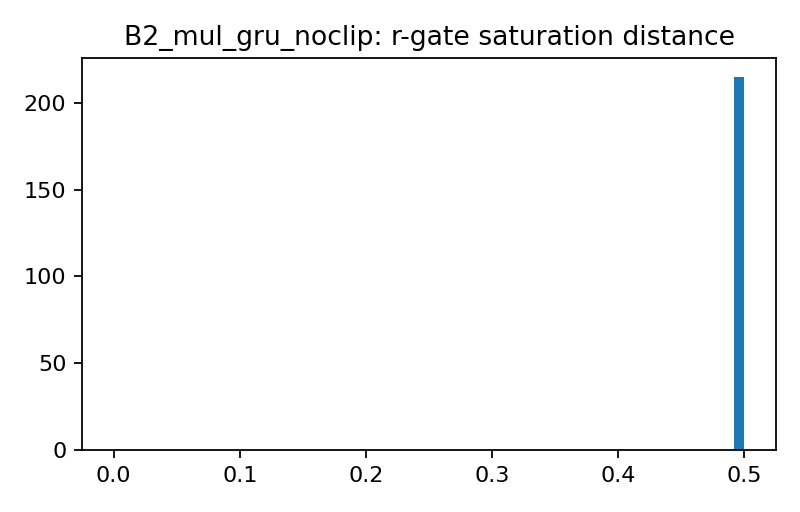
\includegraphics[width=0.48\textwidth]{../runs/figures/B2_mul_gru_noclip_rsat_hist.png}
\caption{GRU gate saturation-distance histograms (update and reset gates).}
\end{figure}
\paragraph{Observation}
On multiplication with GRU, gradients are also strongly vanishing and hidden saturation distance is very high. Gate histograms show update gate relatively more saturated than reset gate. The validation-error curve is slightly better than B1, with best error around 24.25\%.

\section{Required Questions}
\begin{enumerate}
\item \textbf{Gradient histogram interpretation.}
A1 shows comparatively larger gradients with occasional explosive behavior; A2/A3 are shifted left but controlled by clipping; A4 is more vanishing than A1--A3; A5 shifts back right compared to A4 due to clipping-stabilized dynamics. B1 and B2 are both strongly vanishing.

\item \textbf{Hidden saturation-distance interpretation and relation to gradients.}
A1 has strong hidden saturation and unstable gradients. A2/A3 reduce hidden saturation substantially. However, B1/B2 demonstrate that vanishing can still occur even when hidden units are far from saturation (sat means near 0.94--0.99). So saturation is related but not sufficient to explain all gradient behavior.

\item \textbf{Clipping vs no clipping.}
For RNN memorization (A1 vs A2/A3), clipping drastically changes behavior: huge pre-clip norms are rescaled to near cutoff, $\rho$ drops from very large (A1) to near 1, and hidden saturation decreases strongly. For GRU memorization (A4 vs A5), clipping reduces $\rho$ and makes gradients less vanishing while keeping training numerically stable.

\item \textbf{RNN vs GRU comparison and gate behavior.}
On memorization, GRU no-clip (A4) avoids the extreme $\rho$ explosion of A1 but still exhibits vanishing-through-time. Gate histograms indicate update gate is often near saturation while reset gate remains mostly unsaturated. On multiplication (B1 vs B2), both vanish strongly; GRU is slightly better in valid error but still fails to fully solve long-range dependency under this setup. This is a GRU failure mode: gating helps stability but does not guarantee non-vanishing gradients in all regimes.

\item \textbf{$\rho(W_{hh})$ trends and correlation.}
Higher $\rho$ is associated with instability/explosive tendencies (A1 with $\rho\approx14.2$). Clipping keeps $\rho$ around 1-1.3 (A2/A3/A5), corresponding to controlled dynamics. Very low $\rho$ (B2 around 0.08) aligns with strongly contractive dynamics and severe vanishing.
\end{enumerate}

\section{Notes}
For memorization (classification), valid error is strict sequence-level error under report=all. For multiplication (regression), interpret valid error together with valid nll and threshold-based errors printed in logs.

\section{Appendix: Commands}
Exact experiment commands are provided in \texttt{runs/commands\_ran.txt}.

\section{Appendix: Final Submission Structure}
The final submission package contains:
\begin{itemize}
\item \textbf{Code:} \texttt{model.py}, \texttt{train.py}
\item \textbf{Analysis tool:} \texttt{analyze\_results.py}
\item \textbf{Report:} \texttt{report/pa2\_report.pdf} (and source \texttt{report/pa2\_report.tex})
\item \textbf{Required logs:} A1--A5, B1--B2 log files under \texttt{runs/logs/}
\item \textbf{Required run outputs:} A1--A5, B1--B2 \texttt{\_final\_state.npz} files under \texttt{runs/npz/}
\item \textbf{Command log:} \texttt{runs/commands\_ran.txt}
\item \textbf{AI chat links:} \url{https://chatgpt.com/share/69b28578-85e4-800e-b29d-0f3795efa7d7}
\end{itemize}

\end{document}
